\chapter{Définitions Basiques et Exemples}

Les graphes font partie des structures abstraites les plus fondamentales en mathématique discrète. Ils modélisent les situations où des objets sont en relation, et ont donc de nombreuses applications en ingénierie : informatique (réseaux, automates, intelligence artificielle, ...), sciences physiques (transport, optimisation, liaisons chimiques, . . .), sciences de l’information (communication, trafic, . . .), biologie (épi- démiologie, . . .), etc.

Le but de cette première section est d’introduire le vocabulaire de base de la théorie des graphes.
\section{Graphes}

\subsection{Graphes non-orientés} % (fold)
\label{sub:Graphes non-orientés}

% subsection Graphes non-orientés (end)
\begin{Definition}[colbacktitle=red!75!black]{Graphe, Sommet, Arête}{}
Un \textbf{graphe} $G = (S,A)$ est la donnée de deux ensembles :
\begin{itemize}
    \item Un ensemble fini $S$ qu'on appelle l'ensemble des \textbf{sommets}.
    \item $A \subset  \{ \alpha \in \mathcal{P} (S),\; \mathrm{card} (\alpha)=2 \}$ qu'on appelle l'ensemble des \textbf{arêtes}.

        On dit que chaque arête $\{s, s'\}$  \textbf{relie} les sommets $s$ et s', ou que les osmmets $s$ et $s'$ sont les  \textbf{extrémités} de l'arête $\{s, s'\}$
\end{itemize}
\end{Definition}
\begin{Example}{Graphe}{}
\[
    S = \{a,b,c,d\},\; A = \{\{a,b\}, \{a,c\}, \{a,d\},\{b,c\}, \{c,d\}\}
\]
$G = (S,A)$ est un exemple de graphe qu'on peut représenter à l'aide de schéma suivant : 

\begin{center}
    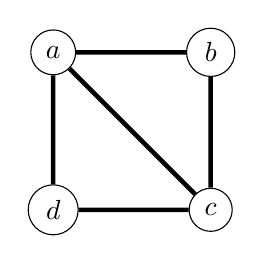
\begin{tikzpicture}
        \tikzstyle{every node}=[draw,shape=circle];
        %\node (name) at (theta:r) [label={text1}] {text2};
        %\draw [option] ...
        %...;
        \node (a) at (-1,1) {$a$};
        \node (d) at (-1,-1) {$d$};
        \node (b) at (1,1) {$b$};
        \node (c) at (1,-1) {$c$};
        \draw[ultra thick] (a)--(b)
        (a)--(c)
        (a)--(d)
        (b)--(c)
        (c)--(d);
    \end{tikzpicture}
\end{center}
\end{Example}

Ainsi un même graphe peut être représenté par des schémas différents. Un schéma n'est pas une figure géométrique. Les seules informations importantes à lire sur le schéma sont les sommets et les arêtes mais pas leur position.

\begin{note}

\begin{itemize}
    \item Dans un graphe, on n'autorise pas les \textbf{boucles} (une arête partout reliant un sommet à lui même) ni les \textbf{arêtes multiples} (au moins deux arrêtes qu'reliant les mêmes sommets).
    \item Sinon, on parle de \textbf{multigraphe}. Dans ce cours, on étudiera seulement les graphes (on dit aussi \textbf{graphes simples}).
\end{itemize}
\end{note}

\begin{Definition}[colbacktitle=red!75!black]{Ordre et taille du graphe}{}
    Soit $S$ un ensemble de sommets. On note $n = \mathrm{card} (S)$ l'\textbf{ordre du graphe}, et $\mathrm{car d}(A)$ d'arêtes la \textbf{taille}.

\end{Definition}

\begin{Prop}{Nombre de graphes possibles d'ordre $n$}{}
On sait que 
\[
  \mathrm{car d}\{x \in \mathcal{P} (S), \mathrm{card}(x) =2 \} = \binom{n}{2} = \frac{n(n-1)}{2} 
\]
et que \[
    A \subset  \{ \alpha \in \mathcal{P} (S),\; \mathrm{car d}(\alpha) =2 \}
\]

Il y a donc au total $2^{n(n-1) /2}$ graphes possibles d'ordre  $n$.
\end{Prop}

\begin{Example}{}{}
    Pour $n = 10$ sommets, on obtient $2^{n(n-1)/2} = 2^{45} \approxeq 3,5 \times 10^{10}$ graphes possibles d'ordre 10.
\end{Example}

\begin{Definition}[colbacktitle=red!75!black]{Graphe Complet, Graphe Linéaire, Graphe Cyclique}{}

\begin{itemize}
    \item \textbf{Graphe complet}, $K_n$
        Soit $n \in \mathbb{N} ^*$, le \textbf{graphe complet} d'ordre $n$, noté $K_n$, est le graphe $G=(S,A)$ donné par :
 \[
     S = \{1,2,\ldots,n\},\; A = \{ \alpha \in \mathcal{P} (S) , \mathrm{car d} ( \alpha ) =2\}
\]

Autrement dit, $\mathrm{car d} (A)$, qui est le nombre d'arêtes qu'on appelle la \textbf{taille du graphe}, est égale à $n(n-1) / 2$ pour le graphe complet d'ordre $n$.
\item \textbf{Graphe Linéaire}, $L_n$

Le \textbf{graphe linéaire} d'ordre $n$, noté $L_n$, est le graphe $G = (S,A)$ donné par :
 \[
     S = \{1, 2, \ldots, n\},\; A = \{\{k, k+1\}, \; k \in [\![1,n]\!]\}
\]

En particulier la taille de $L_n$ est égale à $n-1$.

\item \textbf{Graphe Cyclique}, $C_n$

Le \textbf{graphe cyclique} d'ordre $n$, noté $C_n$, est le graphe $G = (S,A)$ donné par :
 \[
 S = \{1, 2, \ldots, n\},\; A = \{\{k, k+1\}, \; k \in [\![1,n]\!]\} \}\cup \{\{1,n\}\}
\]
\end{itemize}
\end{Definition}

\begin{Example}{Graphe Linéaire}{}
\begin{center}
    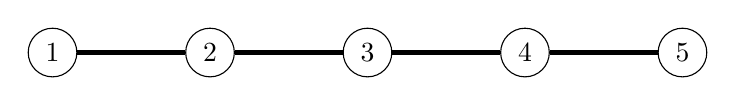
\begin{tikzpicture}
        \tikzstyle{every node}=[draw,shape=circle];
        %\node (name) at (theta:r) [label={text1}] {text2};
        %\draw [option] ...
        %...;
        \node (1) at (-4,0) {1};
        \node (2) at (-2,0) {2};
        \node (3) at (-0,0) {3};
        \node (4) at (+2,0) {4};
        \node (5) at (+4,0) {5};
        \draw[ultra thick] (5)--(4);
        \draw[ultra thick] (4)--(3);
        \draw[ultra thick] (3)--(2);
        \draw[ultra thick] (2)--(1);
    \end{tikzpicture}
\end{center}
\end{Example}

\subsection{Graphe Orienté} % (fold)

% subsection  (end)

\begin{Definition}[colbacktitle=red!75!black]{Graphe Orienté}{}
Un \textbf{graphe orienté} $G=(S,A)$ est la donné :
 \begin{itemize}
    \item Un ensemble fini $S$ de \textbf{sommets}.
    \item $A \subset \{(s,s'), (s,s') \in S^2, s \ne s'\}$ qu'on appelle l'ensemble des \textbf{arcs}.
\end{itemize}

Attention, ce sont les paranthèses que l'on va utiliser.
\end{Definition}



\begin{Example}{Graphe orienté}{}
\[
    S = \{a,b,c\}, \; A = \{(a,b),(a,c),(b,a),(b,c)\}
\]

\begin{center}
    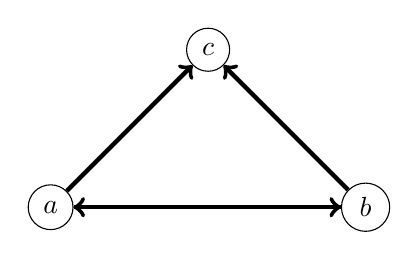
\begin{tikzpicture}
        \tikzstyle{every node}=[draw,shape=circle];
        %\node (name) at (theta:r) [label={text1}] {text2};
        %\draw [option] ...
        %...;
        \node (a) at (-2,0) {$a$};
        \node (b) at (2,0) {$b$};
        \node (c) at (0,2) {$c$};
        \draw[ultra thick, ->] (a)--(b);
        \draw[ultra thick, ->] (a)--(c);
        \draw[ultra thick, ->] (b)--(a);
        \draw[ultra thick, ->] (b)--(c);
        \end{tikzpicture}
\end{center}


\end{Example}

Rappel :
 \begin{itemize}
     \item Pour les paires, $\{s, s'\} = \{s', s\}$ pas d'ordre, les arêtes ne sont pas orientéses.
    \item Pour les couples,  $(s, s') \ne (s', s)$, il y a un ordre. (les arcs sont orientés)
    \item Pour un arc  $(s, s')$,  $s$ est appelé le \textbf{sommet de départ}, $s'$ est appelé \textbf{le sommet d'arrivés}.
 \end{itemize}

\begin{note}
\begin{itemize}
    \item Pour les graphes qui ne sont pas orientés, on parle aussi de \textbf{graphe non-orienté}.
\end{itemize}
\end{note}

\subsection{Graphe Pondéré} % (fold)

% subsection  (end)
\begin{Definition}[colbacktitle=red!75!black]{Graphe Pondéré}{}
Un \textbf{graphe pondéré} est un graphe $G = (S,A)$ qu'on avait d'une  \textbf{fonction de poids} : $f :A \longrightarrow \mathbb{R}$.

Autrement dit, à charque arête $\alpha \in A$ on lui attribue un poids  $f( \alpha )$.

Schématriquement, on place la valeur de $f( \alpha )$ au-dessus de chaque arête.
\end{Definition}

\begin{Example}{Graphe pondéré}{}
Supposons  $S = \{\text{Beijing, Wuhan, Nanjing, Changsha, Shanghai}\}$. La carte des trains à grande vitesse reliant les villes forment un graphe.

En utilisant comme fonction de poids la distance entre deux milles reliées par un train, on obtient un graphe pondéré.
\end{Example}

On peut aussi définir les graphes orientés et pondérés.

\section{Adjacance et degré}

\begin{Definition}[colbacktitle=red!75!black]{Adjacent, Voisin}{}
Deux sommets sont dits \textbf{adjacents} ou \textbf{voisins} s'ils appartiennent à la même arête.
\end{Definition}


\begin{Definition}[colbacktitle=red!75!black]{Degré}{}
Le \textbf{degré} d'un sommet $s$ dans un graphe $G= (S,A)$ est :
\begin{center}
le nombre d'arêtes qui contiennent $s$.
\end{center}
Donc, c'est aussi le nombre cd'arêtes dont $s$ est une extrémité.
\end{Definition}


\begin{Example}{}{}
\begin{center}
    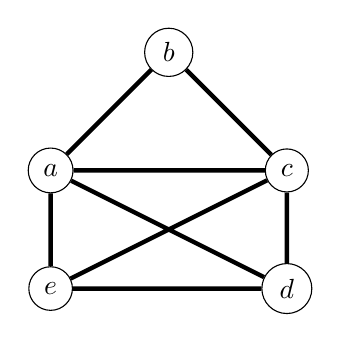
\begin{tikzpicture}[scale=0.5]
        \tikzstyle{every node}=[draw,shape=circle];
        %\node (name) at (theta:r) [label={text1}] {text2};
        %\draw [option] ...
        %...;
        \node (a) at (-3,-3) {$a$};
        \node (b) at (0,0) {$b$};
        \node (c) at (3,-3) {$c$};
        \node (d) at (3,-6) {$d$};
        \node (e) at (-3,-6) {$e$};
        \draw[ultra thick] (a)--(c)
        (a)--(b)
        (b)--(c)
        (c)--(d)
        (c)--(e)
        (e)--(d)
        (a)--(d)
        (a)--(e);
    \end{tikzpicture}
\end{center}
$a$ et $c$ sont adjacents mais $b$ et $d$ ne le sont pas.

On a :
    \[
    \mathrm{deg} (a) = \mathrm{deg} (c) = 4,\; \mathrm{deg} (b) = 2,\; \mathrm{deg} (e) = \mathrm{deg} (d) = 3
    \]
\end{Example}

\begin{Definition}[colbacktitle=red!75!black]{Isolé}{}
Lorsque le degré d'un sommet $s$ est nul, on dit que ce sommet est \textbf{isolé}.
\end{Definition}


\begin{Prop}{Somme de degrés}{}
Pour $\forall s \in S$,  notant $n = \mathrm{card}(S)$
\[
\mathrm{deg}(s) \le \mathrm{card}(S) - 1 = n-1 \implies \boxed{\sum_{s \in S} \mathrm{deg}(s) \le n(n-1)}
\]
Puisque chaque arête contient exactement 2 sommets, la somme des degrés est égale au double de la taille.
 \[
   \boxed{\sum_{s \in S} \mathrm{deg} (s) = 2 \,\mathrm{car d} (A)} \implies \mathrm{card}(A) \le \binom{n}{2}
\]
\end{Prop}


\begin{Corollary}{Lemme des poignés de mains}{}
Le nombre de sommets de degré impaire est pair.
\end{Corollary}


\section{Chemin et connexité}

\begin{Definition}[colbacktitle=red!75!black]{Chemin}{}
Un \textbf{chemin} est de façon équivalente :
\begin{itemize}
    \item Une suite de sommets telle que deux sommets consécutives dans la suite sont adjacents.
    \item Une suite d'arêtes telle que deux arêtes consécutives dans la suite ont un sommet commun.
\end{itemize}
\end{Definition}

\begin{Example}{Chemin}{}
Dans l'exemple précédent,
\begin{itemize}
    \item $(a,b,c,a,e)$ est un chemin. (Un chemin peut passer 2 fois par le même sommet)
    \item $(\{d,c\},\{c,e\}, \{e, c\}, \{c,b\})$ est un chemin. (Un chemin peut passer 2 fois par le même arête)
\end{itemize}
\end{Example}

\begin{Definition}[colbacktitle=red!75!black]{Reliés par un chemin}{}
On dit que deux sommets sont \textbf{reliés par un chemin} s'il existe au moins un chemin dont le premier et le dernier sommet sont les sommet reliés.
\end{Definition}

\begin{Example}{}{}
Dans l'exemple précédent, $b$ et $d$ ne sont pas adjacents mais sont reliés par le chemin $(b,c,d)$
\end{Example}

\begin{Prop}{Reliés par un chemin est une relation d'équivalence}{}
Le fait d'être relié par un chemin est \textit{réflexif}, \textit{symétrique} et \textit{transitif}.

On reconnait une \textbf{relation d'équivalence}.
\end{Prop}

\begin{myproof}
La relation est :
\begin{itemize}
    \item Réflexivité : Un sommet est toujours relié à lui-même par un chemin de 0 arête.
    \item Symétrique : Si $s$ est relié à $s'$ par un chemin alors $s'$ est relié à $s$ par le chemin inverse.
    \item Transitivité : Si $s$ est relié par un chemin à $s'$ et $s'$ est relié par un chemin à $s"$, alors  $s$ est relié par un chemin à $s"$ qu'on obtient en seignant les deux chemins.
\end{itemize}
\end{myproof}

\begin{Definition}[colbacktitle=red!75!black]{Composante Connexe}{}
La \textbf{composante connexe} d'un sommet $s$ est l'ensemble des sommets qui sont reliés à $s$ par un chemin. (c'est à dire la classe d'équivalence pour la relation d'équivalence d'être relié par un chemin)



\end{Definition}


\begin{Example}{Composante Connexe}{}
\begin{center}
    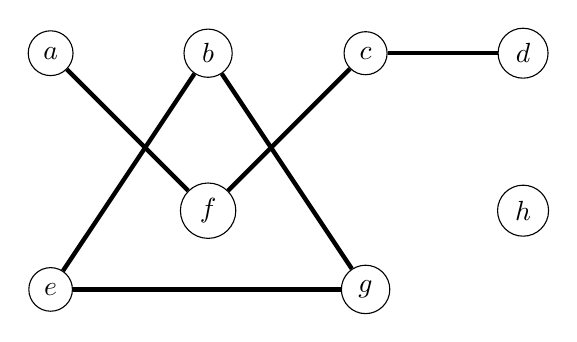
\begin{tikzpicture}
        \tikzstyle{every node}=[draw,shape=circle];
        %\node (name) at (theta:r) [label={text1}] {text2};
        %\draw [option] ...
        %...;
        \node (a) at (-2,2) {$a$};
        \node (b) at (0,2) {$b$};
        \node (c) at (2,2) {$c$};
        \node (d) at (4,2) {$d$};
        \node (e) at (-2,-1) {$e$};
        \node (f) at (0,0) {$f$};
        \node (g) at (2,-1) {$g$};
        \node (h) at (4,0) {$h$};
        \draw[ultra thick] (a)--(f);
        \draw[ultra thick] (e)--(b);
        \draw[ultra thick] (b)--(g);
        \draw[ultra thick] (f)--(c);
        \draw[ultra thick] (c)--(d);
        \draw[ultra thick] (e)--(g);
    \end{tikzpicture}
\end{center}
\begin{itemize}
    \item Il y a 3 \textbf{composantes connexes} : $\{a,c,d,f\}, \; \{b,e,g\}, \{h\}$
    \item $\mathrm{deg} (h) =0$, $h$ est appelé un \textbf{sommet isolé}
    \item La composante connexe d'un sommet isolé contient seulement ce sommet.
\end{itemize}
\end{Example}
\begin{Definition}[colbacktitle=red!75!black]{Graphe connexe}{}
Un graphe est dit \textbf{connexe} s'il \underline{ne contient qu'une seule composante connexe}. C'est-à-dire lorsque pour tout couple de sommets, il existe au moins un chemin qui les relie.
\end{Definition}

\begin{Example}{}{}
    L'exemple précédent n'est pas un graphe connexe. Mais il peut le devenir si on ajoute les arêtes $\{a,b\}$ et $\{g,h\}$
\end{Example}

\begin{Example}{}{}
Les graphes $K_n$, $L_n$ et $C_n$ sont connexes.
\end{Example}


\begin{Prop}{}{} \label{Relation-connexité}
  Si un graphe $G= (S,A)$ est connexe, alors :
  \[
    \boxed{\mathrm{card} (A) \ge  \mathrm{card} (S) - 1 }
  \]

  La réciproque est fausse.

  \end{Prop}

  \begin{myproof}
  On raisonne par récurrence sur l'ordre de $G$, c'est-à-dire sur $n = \mathrm{card} (S)$.
  La réciproque est fausse.
  \begin{itemize}
      \item Initialisation

          Si $n=1$, on a 1 seul sommet et 0 arrête.
          Si $n=2$, on a 2 sommets, nécessairement 1 arrête pour être connexe.

      \item Hérédité

          On suppose que la propriété est vraie pour tous les graphes connexes d'ordre $n$.

          Soit $G = (S,A)$ un graphe connexe d'ordre $n+1$, c'est-à-dire  $\mathrm{card} (S) = n+1$

           D'après la connexité de $G$, on sait qu'il n'y a pas de point isolé, c'est-à-dire, $\forall  s\in S, \mathrm{deg} (s) \ge 1$.

           \begin{itemize}
               \item 1er cas : Il existe au moins un sommet de degré 1, c'est-à-dire, $\exists  s \in S, \mathrm{deg} (s) = 1$, on considère le graphe $G'= (S',A')$ qu'on obtient en retirant le sommet  $s$ de $G$ et l'unique arrête partant de $s$.

                   Donc $S'= S \backslash \{s\}$, et  $\mathrm{car d}(A') = \mathrm{car d}(A) - 1 $ 

                   Par construction, $G' = (S', A')$ est encore un graphe connexe d'ordre $(n+1)-1=n$. 

                   D'après l'hypothèse de récurrence, on sait que \[
                   \mathrm{car d}(A') \ge  \mathrm{ car d}(A) - 1 = n-1  
                   \]
                   Donc $\mathrm{car d}(A) \ge n$
              \item 2ème cas : Tous les sommets sont de degré supérieur ou égal à $\alpha$, c'est-à-dire  $\forall  s \in S$, $\mathrm{deg} (s) \ge 2$ .

                  On sait que : $\sum_{s \in S} \mathrm{deg} (s) = 2\times \mathrm{car d}(A) $, 

                  Donc : \[
                  \mathrm{car d} (A) = \frac{1}{2} \sum_{s \in S} \mathrm{deg} (s) \ge  \frac{1}{2} \sum_{s \in S}2 = \mathrm{car d} (S) = n
                  \]

                  
           \end{itemize}
          \item Conclusion

              Dans les deux cas, $\mathrm{car d} (A) \ge \mathrm{car d}(S)-1 $, donc la propriété est vraie au rang $n+1$ lorsqu'elle est vraie au rang $n$.

                  On en déduit qu'elle est vraie pour tout $n \in \mathbb{N} ^{*}$ d'après le principe de récurrence.
  \end{itemize}

  \end{myproof}

  \begin{Example}{Contre-exemple}{}

  On considère le graphe $K_3$ auquel on rajoute un point isolé.
  \begin{center}
      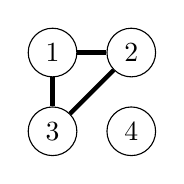
\begin{tikzpicture}
          \tikzstyle{every node}=[draw,shape=circle];
          %\node (name) at (theta:r) [label={text1}] {text2};
          %\draw [option] ...
          %...;
          \node (1) at (0,0) {1};
          \node (2) at (1,0) {2};
          \node (3) at (0,-1) {3};
          \node (4) at (1,-1) {4};
          \draw[ultra thick] (1)--(2);
          \draw[ultra thick] (2)--(3);
          \draw[ultra thick] (1)--(3);
      \end{tikzpicture}
  \end{center}
  $\mathrm{car d}(S) = 4,\; \mathrm{car d}(A) = 3$ mais le graphe n'est pas connexe.
  \end{Example}

  \begin{Definition}[colbacktitle=red!75!black]{Chemin élementaire et simple}{}
  Un \textbf{chemin} est dit :
  \begin{itemize}
      \item \textbf{Élémentaire}
          
          lorsqu'il ne passe pas deux fois par le même sommet, c'est-à-dire que les sommets du chemin sont deux à deux différents.

      \item \textbf{Simple}

          lorsqu'il ne passe pas deux fois par la même arrête, c'est-à-dire que les arrêtes du chemin sont deux à deux différentes.
  \end{itemize}
  \end{Definition}

  \begin{Example}{$K_5$}{}

  On considère le chemin $(1, 2, 3, 1, 4, 5, 1)$ ou de manière équivalente : $$(\{1,2\},\{2, 3\},\{3, 1\},\{1, 4\}, \{4, 5\}, \{5, 1\})$$ (C'est un chemin \textbf{simple} mais pas \textbf{élémentaire})

  \begin{center}
      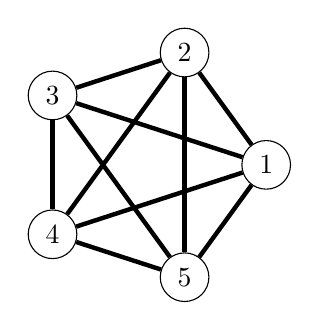
\begin{tikzpicture}[scale=0.5]
          \tikzstyle{every node}=[draw,shape=circle];
          %\node (name) at (theta:r) [label={text1}] {text2};
          %\draw [option] ...
          %...;
          \node (1) at (0:3) {1};
          \node (2) at (72:3) {2};
          \node (3) at (2*72:3) {3};
          \node (4) at (3*72:3) {4};
          \node (5) at (4*72:3) {5};
          \draw[ultra thick] (1)--(2);
          \draw[ultra thick] (2)--(3);
          \draw[ultra thick] (3)--(4);
          \draw[ultra thick] (4)--(5);
          \draw[ultra thick] (5)--(1);
          \draw[ultra thick] (2)--(5);
          \draw[ultra thick] (1)--(3);
          \draw[ultra thick] (2)--(4);
          \draw[ultra thick] (1)--(4);
          \draw[ultra thick] (3)--(5);
      \end{tikzpicture}
  \end{center}
  \end{Example}

  \section{Cycles et Acyclique}

  \begin{Definition}[colbacktitle=red!75!black]{Cycles, Acyclique}{}
  Dans un graphe, un \textbf{cycle} est \underline{un chemin simple d'au moins 3 arrêtes qui relie un sommet à lui-même}, l'ordre d'un \textbf{cycle} est son nombre de sommets. 

  En revanche, un graphe est dit \textbf{acyclique} s'il ne contient aucun cycle. 
  \end{Definition}

  \begin{Example}{$L_n, C_n$}{}
  Le graphe $L_n$ est acyclique.
  \begin{center}
      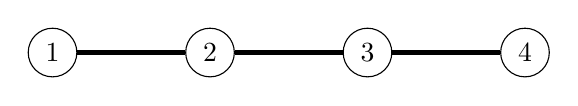
\begin{tikzpicture}
          \tikzstyle{every node}=[draw,shape=circle];
          %\node (name) at (theta:r) [label={text1}] {text2};
          %\draw [option] ...
          %...;
          \node (1) at (-2,0) {1};
          \node (2) at (0,0) {2};
          \node (3) at (2,0) {3};
          \node (4) at (4,0) {4};
          \draw[ultra thick] (1)--(2)
          (2)--(3)
          (3)--(4);
      \end{tikzpicture}

  \end{center}
      Le graphe $C_n$ n'est pas acyclique.

  \begin{center}
      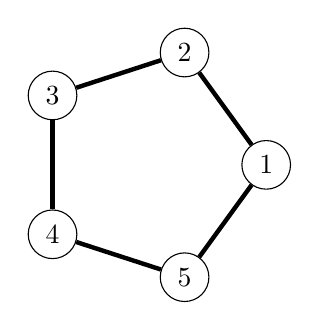
\begin{tikzpicture}[scale=0.5]
          \tikzstyle{every node}=[draw,shape=circle];
          %\node (name) at (theta:r) [label={text1}] {text2};
          %\draw [option] ...
          %...;
          \node (1) at (0:3) {1};
          \node (2) at (72:3) {2};
          \node (3) at (2*72:3) {3};
          \node (4) at (3*72:3) {4};
          \node (5) at (4*72:3) {5};
          \draw[ultra thick] (1)--(2);
          \draw[ultra thick] (2)--(3);
          \draw[ultra thick] (3)--(4);
          \draw[ultra thick] (4)--(5);
          \draw[ultra thick] (5)--(1);
      \end{tikzpicture}
  \end{center}

  Le graphe $K_n$ n'est pas acyclique.

      
  \begin{center}
      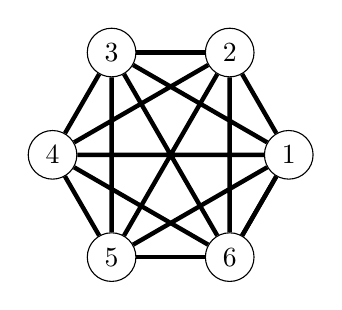
\begin{tikzpicture}[scale=0.5]
          \tikzstyle{every node}=[draw,shape=circle];
          %\node (name) at (theta:r) [label={text1}] {text2};
          %\draw [option] ...
          %...;
          \node (1) at (0:3) {1};
          \node (2) at (60:3) {2};
          \node (3) at (2*60:3) {3};
          \node (4) at (3*60:3) {4};
          \node (5) at (4*60:3) {5};
          \node (6) at (5*60:3) {6};
          \draw[ultra thick] (1)--(2);
          \draw[ultra thick] (2)--(3);
          \draw[ultra thick] (3)--(4);
          \draw[ultra thick] (4)--(5);
          \draw[ultra thick] (5)--(6);
          \draw[ultra thick] (6)--(1);
          \draw[ultra thick] (1)--(3)
          (1)--(4)
          (1)--(5)
          (1)--(6)
          (2)--(4)
          (2)--(5)
          (2)--(6)
          (3)--(5)
          (3)--(6)
          (4)--(6);
      \end{tikzpicture}
  \end{center}

  Il contient des cycles d'ordre 3, 4, 5 et 6. ($n \ge 3$) 

  ($K_1$ et $K_2$ sont acycliques)
  \end{Example}

  \begin{Prop}{}{}
  Soit $G = (S,A)$ un graphe, si tous les sommets de $G$ sont de degré supérièur ou égal à 2 (c'est-à-dire $\forall  s \in S, \mathrm{deg}(s) \ge  2$), alors $G$ contient au moins un cycle, donc $G$ n'est pas acyclique.
  \end{Prop}

  \begin{myproof}
  On va construire un cycle à l'aide d'un algorithme, et on va construire par récurrence une list de sommets $s_0, s_1, \ldots, s_k$.

  \begin{itemize}
      \item On choisit arbitrairement un sommet $s_0$
      \item Pour chaque $s_{i+1}$, on choisit un sommet adjacent à $s_i$ qu'on n'a pas déjà choisi dans la liste avant.
      \item L'algorithme s'arrête dès que tous les voisins de $s_k$ ont déjà été choisi dans la liste.
  \end{itemize}

  Par hypothèse, $\mathrm{deg} (s_k) \ge 2$, donc il existe au moins un autre voisin que $s_{k-1}$ de $s_k$ \textit{dans la liste}. On note cet autre voisin $s_j$ où  $j <k-1$. (Propriété de récurrence)

  On considère le chemin \[
      (s_k, s_j, s_{j+1},\ldots, s_{k-1}, s_k)
  \]

  Par construction, c'est un cycle !! Donc $G$ n'est pas acyclique.
  \end{myproof}  

  \begin{Corollary}{Propriété d'acyclique}{} \label{Cor:Pro d'acyclique}
  Si u graphe $G = (S,A)$ est \textbf{acyclique} alors :
  \[
  \boxed{  \mathrm{card}(A) \le \mathrm{card}(S) - 1}
  \]

  La réciproque est fausse.
  \end{Corollary}

  \begin{myproof}
  On raisonne par récurrence sur l'ordre de $G$, qu'on note $n = \mathrm{car d}(S)$

  \begin{itemize}
      \item Initialisation : La propriété est évidente pour $n=1$ ou $n=2$

      \item Hérédité : On suppose que la propriété est vraie pour tous les graphes d'ordre $n$.

          Soit $G = (S,A)$ un graphe acyclique d'ordre $n+1$, d'après la propriété précédante, on sait qu'il existe au moins un sommet de degré 0 ou 1, c'est-à-dire  
          \[
              \exists  s \in S, \; \mathrm{deg} (S) \in \{0,1\}
          \]
         
          On considère le graphe $G' = (S', A')$ qu'on obtient en retirent le sommet  $s$ du graphe $G$ et, si $\mathrm{deg} (s)=1$, l'unique arrête qui part de $s$. 

          Donc $S'= S \backslash \{s\}$, et 
          \[
          \mathrm{car d}(A') = \begin{cases}
              \mathrm{car d}(A) \text{ si } \mathrm{deg} (s) = 0 \\
              \mathrm{car d}(A) - 1 \text{ si } \mathrm{deg}(s) = 1  
          \end{cases} 
          \]
         $\mathrm{car d}(A') \ge   \mathrm{car d} (A) -1$.

         Par construction $G'$ est un graphe acyclique d'ordre  $n$. Par hypothèse de récurrence, $\mathrm{car d}(A') \le  n-1$, par conséquent $\mathrm{car d} (A) \le n$ 

      \item Concclusion : La propriété est vraie pour tout ordre $n \in \mathbb{N} ^{*}$ d'après la principe de récurrence
  \end{itemize}

  \begin{Example}{Contre-Exemple}{}
  Si on considère le graphe $K_3$ auquel on ajouter un point isolé,
  \begin{center}
      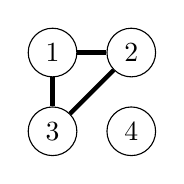
\begin{tikzpicture}
          \tikzstyle{every node}=[draw,shape=circle];
          %\node (name) at (theta:r) [label={text1}] {text2};
          %\draw [option] ...
          %...;
          \node (1) at (0,0) {1};
          \node (2) at (1,0) {2};
        \node (3) at (0,-1) {3};
        \node (4) at (1,-1) {4};
        \draw[ultra thick] (1)--(2);
        \draw[ultra thick] (2)--(3);
        \draw[ultra thick] (1)--(3);
    \end{tikzpicture}
\end{center}
$\mathrm{car d}(S) = 4,\; \mathrm{car d}(A) = 3$ mais le graphe n'est pas acyclique.
\end{Example}
\end{myproof}

\section{Arbres}

\begin{Definition}[colbacktitle=red!75!black]{Arbres}{}
Un \textbf{arbre} est un graphe connexe et acyclique.
\begin{itemize}
    \item Les sommets de degré 1 sont appelés des \textbf{feuilles}
    \item Les arbres sommets (de degré supérieur ou égal à 2) sont appelés des \textbf{noeuds}.
\end{itemize}
\end{Definition}

\begin{Example}{Arbre}{}
\begin{center}
  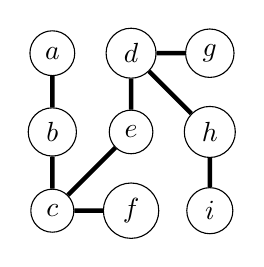
\begin{tikzpicture}
    \tikzstyle{every node}=[draw,shape=circle];
    %\node (name) at (theta:r) [label={text1}] {text2};
    %\draw [option] ...
    %...;
    \node (a) at (-1,+1) {$a$};
    \node (b) at (-1,0) {$b$};
    \node (c) at (-1,-1) {$c$};
    \node (d) at (0,+1) {$d$};
    \node (e) at (0,0) {$e$};
    \node (f) at (0,-1) {$f$};
    \node (g) at (1,1) {$g$};
    \node (h) at (1,0) {$h$};
    \node (i) at (1,-1) {$i$};
    \draw[ultra thick] (a) -- (b)
    (b) -- (c)
    (c) -- (e)
    (c) -- (f)
    (e) -- (d)
    (d) -- (g)
    (d) -- (h)
    (h) -- (i);
  \end{tikzpicture}
\end{center}
\end{Example}

\begin{Prop}{}{}
Si $T = (S,A)$ est un \textbf{arbre} alors \[
\mathrm{card} (A) = \mathrm{card} (S) - 1
\]
\end{Prop}

\begin{myproof}{}{}
  Récurrence. 

  Note : On peut toujours trouver une feuille dans l'arbre car finie. On la note $F$. 

  En supprimant $F$, il reste une arbre que l'on connaît. De plus, il faut ajouter l'arête connectant $F$ et son \textbf{parent} (définira au-dessous)
\end{myproof}





\begin{Theorem}{Caractérisation des Arbres}{}
Soit $G=(S,A)$ un graphe. Les propositions suivantes sont équivalentes : 
\begin{enumerate}
  \item $G$ est un arbre 
  \item $G$ est connexe et $\mathrm{card}(A) = \mathrm{card}(S)-1$ 
  \item $G$ est \textbf{connexe minimal}  : si on la retire une arête, il n'est plus connexe. 
  \item $G$ est acyclique et $\mathrm{card}(A) = \mathrm{card}  (S)-1$    
  \item $G$ est \textbf{acyclique maximal} : si on lui rajoute une arête, il n'est plus acyclique. 
  \item Pour tout couple de sommets, il existe un unique chemin simple les reliant.
\end{enumerate}
\end{Theorem}

\begin{myproof}
  On montre $(1) \implies (2) \implies (3)$. On peut montrer aussi que $(1) \implies (4) \implies(5)$. 

  \begin{itemize}

      \item $(2) \implies (3)$ car si $G$ reste connexe on lui retirant une arête alors $\mathrm{card} (A) - 1 \ge \mathrm{card} (S) - 1$ donc $\mathrm{card} (A) \ge \mathrm{card} (S) > \mathrm{card}(S) - 1$ ce qui contredit $(2)$. (Voir \ref{Relation-connexité})

      \item De même on montre $(4) \implies(5)$ par l'absurde. 
  

      \item $(3) \implies(1)$ : On suppose que $G$ est connexe minimal. Par l'absurde, supposons que $G$ n'est pas acyclique, donc qu'il contient un cycle. Donc si on retire une arête de ce cycle, le graphe reste connexe. Ce qui contradit que $G$ est connexe minimal. Donc $G$ est acyclique, c'est un arbre.

      \item $(5) \implies (1)$ : On suppose que $G$ est acyclique minimal. Par l'absurde, supposons que $G$ n'est pas connexe, donc qu'il admet plusieurs composantes connexes. Donc, si on ajoute une arête reliant un sommet d'une composante connexe à un sommet d'une autre composante connexe, le graphe reste acyclique. Ce qui contradit que $G$ est acyclique maximal. Donc $G$ est connexe, c'est un arbre.

      \item $(1) \implies (6)$ : Soient $s$ et $s'$ deux sommets de $G$, puisque $G$ est connexe, il existe au moins un chemin (simple) qui relie $s$ et $s'$. S'il existe au moins deux chemins qui reliant $s$ et $s'$ alors on pourrait créer un cycle ce qui contrredit que $G$ est acyclique.

      \item $(6) \implies (1)$ : De même. Si tout couple de sommets peut être relié par un chemin alors $G$ est connexe. Si $G$ n'était pas acyclique, on pourrait relier deux sommets par au moins deux chemins ce qui cest absurde.  

  \end{itemize}
\end{myproof}

\begin{note}
En pratique, pour montrer qu'un graphe est un arbre, il suffit de montrer qu'il est connexe ou bien acyclique (un seul suffit) puis de vérifier que $\mathrm{card} (A) = \mathrm{card} (S) - 1$.
\end{note}

\begin{Corollary}{}{}
Tout arbre admet au moins 2 feuilles.
\end{Corollary}

\begin{myproof}
  Soit $G = (S,A)$ un arbre. On note $F$ son nombre de feuilles, c'est-à-dire $F = \mathrm{card} \left\{ s \in S,\; \mathrm{deg}(s) = 1  \right\}$  

  On sait que : $2 \mathrm{card} (A) = \sum _{s \in S} \mathrm{deg} (s)$ et $\mathrm{card} (A) = \mathrm{card} (S) -1$

  On note $n = \mathrm{card} (S)$ l'ordre du graphe. Donc, 
  \begin{align*}
    2(n-1) &= \sum _{s \in S} \mathrm{deg} (s) \\ 
           &= \sum _{s \text{ feuilles de }G} \mathrm{deg} (s) +  \sum _{s \text{ noeuds de }G} \mathrm{deg} (s) \\ 
           &= F + \sum _{\mathrm{card} = n-F}  \mathrm{deg} (s) \\ 
           &= F + 2(n-F)
  \end{align*}
\end{myproof}

\begin{Definition}[colbacktitle=red!75!black]{Arbre enraciné}{}
Un \textbf{arbre enraciné} est un arbre dans lequel on choisit un sommet particulier qu'on appelle sa \textbf{racine}.

Un arbre enraciné est muni d'une \textbf{fonction hauteur} $h : S \to \mathbb{N}$ qui à chaque sommet $s$ lui associé sa hauteur $h(s)$ égale à la longueur de l'unique chemin simple qui relie $s$ à la racine.
\end{Definition}

\begin{Example}{Arbre enraciné}{}
De l'arbre, 
\begin{center}
  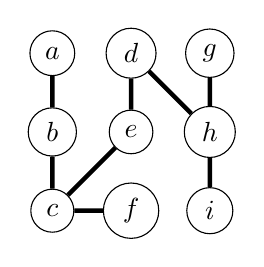
\begin{tikzpicture}
    \tikzstyle{every node}=[draw,shape=circle];
    %\node (name) at (theta:r) [label={text1}] {text2};
    %\draw [option] ...
    %...;
    \node (a) at (-1,+1) {$a$};
    \node (b) at (-1,0) {$b$};
    \node (c) at (-1,-1) {$c$};
    \node (d) at (0,+1) {$d$};
    \node (e) at (0,0) {$e$};
    \node (f) at (0,-1) {$f$};
    \node (g) at (1,1) {$g$};
    \node (h) at (1,0) {$h$};
    \node (i) at (1,-1) {$i$};
    \draw[ultra thick] (a) -- (b)
    (b) -- (c)
    (c) -- (e)
    (c) -- (f)
    (e) -- (d)
    (h) -- (g)
    (d) -- (h)
    (h) -- (i);
  \end{tikzpicture}
\end{center}

on a : 
\begin{center}
  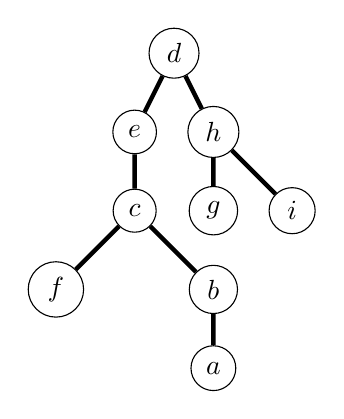
\begin{tikzpicture}
    \tikzstyle{every node}=[draw,shape=circle];
    %\node (name) at (theta:r) [label={text1}] {text2};
    %\draw [option] ...
    %...;
    \node (d) at (0,0) {$d$};
    \node (e) at (-0.5,-1) {$e$};
    \node (h) at (0.5,-1) {$h$};
    \node (g) at (0.5,-2) {$g$};
    \node (i) at (1.5,-2) {$i$};
    \node (c) at (-0.5,-2) {$c$};
    \node (f) at (-1.5,-3) {$f$};
    \node (b) at (0.5,-3) {$b$};
    \node (a) at (0.5,-4) {$a$};


    \draw[ultra thick] (d)--(h) 
    (d)--(e)
    (d)--(h)
    (h)--(g)
    (h)--(i)
    (e)--(c)
    (c)--(f)
    (c)--(b)
    (b)--(a);
  \end{tikzpicture}
\end{center}

\end{Example}

\begin{Definition}[colbacktitle=red!75!black]{Enfants et descendants}{}
Dans un arbre enraciné, on définit pour chaque sommet $s$ : 
\begin{itemize}
  \item Ses \textbf{enfants} : les sommets reliés par une arête à $s$ de hauteur $h(s) + 1$  
  \item Ses \textbf{descendants} : les composantes connexes de $S \backslash \{s\}$ qui ne contient pas la racine. 
  \item Ses \textbf{parents} (sauf pour la racine) : le sommet relié par une arête à $s$ de hauteur $h(s)-1$  
  \item Ses \textbf{ancêtres} : les sommets de l'unique chemin qui relie $s$ à la racine (sauf $s$) 
\end{itemize}
\end{Definition}

\begin{Definition}[colbacktitle=red!75!black]{Forêt}{}
Une \textbf{forêt} est un graphe acyclique (pas nécessairement connexe), autrement dit un graphe dont toutes les composantes connexes sont des arbres.
\end{Definition}

\begin{Prop}{}{}
Soit $G = (S,A)$   une forêt, alors \[
\mathrm{card}(A) = \mathrm{card}  (S) - K
\]
où $K$   est le nombre de composantes connexes de $G$.
\end{Prop}

\begin{myproof}
  On note $\left( G_i = (S_i, A_i) \right) _{i \in [\![1,n]\!]}$, les composantes connexes de $G$. Puisque $G_i$ est un arbre, on a $\mathrm{card}(A_i) = \mathrm{card}(S_i) - 1$  

  Donc, \[
  \sum_{n=1}^{k} \mathrm{card} (A_n) = \sum_{n=1}^{K} (\mathrm{card} (S_i)-1) \implies \mathrm{card} (A) = \mathrm{card} (S) - K
  \]
\end{myproof}

\begin{Definition}[colbacktitle=red!75!black]{Sous-graphe}{}
  \begin{itemize}
    \item Soit $G=(S,A)$ un graphe, un \textbf{sous-graphe} de $G$ est un graphe $G'= (S', A')$ tel que $S' \subset S$ et $A' \subset A$, autrement dit un sous-graphe est un graphe obtenu en supprimant des sommets ou des arêtes. 
    \item Un \textbf{sous-graphe partiel} est un sous-graphe $G'=(S', A')$ tel que $S' =S$, autrement dit un sous-graphe partiel est un graphe obtenu en supprimant seulement des arrêtes.
    \item Un \textbf{sous-graphe induit} est un sous-graphe $G' = (S', A' )$   tel que $A' = \{\{s, s'\}\in A, \; (s, s') \in S'^{2}\}$ , autrement dit un sous-graphe induite est un sous-graphe obtenu en supprimant seulement des sommets.
  \end{itemize}

\end{Definition}

\begin{Definition}[colbacktitle=red!75!black]{Arbre couvrant}{}
Soit $G = (S,A)$, un \textbf{arbre couvrant} de $G$ est un sous-graphe ppartiel de $G$ qui est un arbre.
\end{Definition}

\begin{Prop}{}{}
Soit $G = (S,A)$ un graphe, alors $G$ est connexe si et seulement si $G$ admet un arbre convrant.
\end{Prop}

\begin{myproof}
  $(\impliedby)$ On suppose que $G$ admet un arbre couvrent donc tout couple de sommets de $G$ est relié par un chemin d'arêtes de l'arbre, donc par un chemin d'arêtes de $G$, donc $G$ est connexe. 

  $( \implies)$  Soit $G$   un graphe connexe. Si $G$   est acyclique alors $G$   est un arbre et c'est fini. Si $G$  contient des cycles, on supprime une arête de chaque cycle. 

  On obtient un graphe partiel qui est touours connexe et acyclique, donc un arbre couvrant.
\end{myproof}
